The given equation of the curve:
\begin{align}
    \vec{x^Tx}=25\label{eq:solutions/3/2/1/a/giveneqn}
\end{align}
The general equation of a second degree can
be expressed as:
\begin{align}
    \vec{x^TVx}+2\vec{u^Tx}+f=0 \label{eq:solutions/3/2/1/a/geneqn}
\end{align}
Comparing \eqref{eq:solutions/3/2/1/a/geneqn} with \eqref{eq:solutions/3/2/1/a/giveneqn}:\\
\begin{align}
    \vec{V} =  \vec{I},\vec{u}=\myvec{0\\0} and f=-25 
\end{align}
For $\vec{V}$ =  $\vec{I}$, \eqref{eq:solutions/3/2/1/a/geneqn} represents a circle. \quad$\vec{c}$ represent the center , r the radius  and $\vec{q}$ the point of contact of the tangent to the circle .\\
The center and radius is given by:
\begin{align}
\vec{c}=-\vec{u}=\myvec{0\\0}\label{eq:solutions/3/2/1/a/ceneqn}\\
r=\sqrt{\vec{u^Tu}-f}=\sqrt{0-(-25)}=5
\end{align}

The given point of contact
\begin{align}
 \vec{q}=\myvec{3\\4} \label{eq:solutions/3/2/1/a/coord}  
\end{align}
The direction vector of the line joining the point $\vec{q}$ and the center $\vec{c}$ is:
\begin{align}
 \vec{n}= \vec{q}-\vec{c}\\
  \Longrightarrow\vec{n}= \vec{q}+\vec{u}=\myvec{3\\4}
\end{align}
The vector $\vec{n}$ is  normal to the tangent of the circle, drawn at $\vec{q}$\\
The equation of the tangent is
\begin{align}
 \vec{n^T}\myvec{\vec{x}-\vec{q}}=0\\
 \vec{n^T}\vec{x}=c\\
 \end{align}
 where 
 \begin{align}
c=\vec{n^T}\vec{q}\\
  \Longrightarrow c=\myvec{3\quad4}\myvec{3 \\4}=25
 \end{align}
Thus the equation of the tangent to the curve at $\vec{q}$ is
\begin{align}
    \vec{n^T}\vec{x}=25\\
     \Longrightarrow \myvec{3\quad4}\vec{x}=25
\end{align}

\begin{figure}[!]
 \begin{center}
  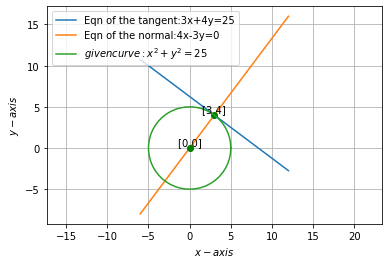
\includegraphics[width=\columnwidth]{solutions/3/2/1/a/assignment5_fig.png}
    \caption{This is the 2D diagram of the given curve  $\vec{x^Tx}=25$ and the tangent to it at $\myvec{3\\4}$}
    \label{eq:solutions/3/2/1/a/myfig:1}
    \end{center}
\end{figure}
